\section{Syntax-Directed Definitions}
A Syntax-Directed Definition (SDD) is a context-free grammar in which:
\begin{itemize}
    \item each symbol can have an associated set of attributes (numbers, types, table references, strings, memory locations, \ldots);
    \item each production can have an associated set of semantic rules (evaluating attributes, interacting with the symbol table, writing lines of intermediate code to a buffer, printing messages, \ldots).
\end{itemize}

\subsection{Inherited and Synthesized Attributes}
A semantic rule associated with a production $A \to XYZ$ can refer only attributes associated with symbols in that production:
\begin{description}
    \item[Inherited Attributes] are evaluated in rules where the associated symbol is on the right side of the production;
    \item[Synthesized Attributes] are evaluated in rules where the associated symbol is on the left side of the production.
\end{description}

\begin{table}[h]
    \centering
    \begin{tabular}{l|l}
        Productions & Semantic Rules \\ \hline
        $L \to Em$ & $print(E.val)$ \\ \hline
        $E \to E_1 + T$ & $E.val = E_1.val + T.val$ \\ \hline
        $E \to T$ & $E.val = T.val$ \\ \hline
        $T \to T_1 \ast F$ & $T.val = T1_.val \ast F.val$ \\ \hline
        $F \to digit$ & $F.val = digit.lexval$
    \end{tabular}
    \caption{SDD example for a desk calculator.}
\end{table}
Each of the non-terminal $E, T, F$ has a single synthesized attribute, named ``val''; the terminal digit has an attribute ``lexval'' which is the integer value returned by the scanner.

\begin{table}[h]
    \centering
    \begin{tabular}{l|l}
        Productions & Semantic Rules \\ \hline
        $D \to TL$ & $L.inh = T.type$ \\ \hline
        $T \to int$ & $T.type = integer$ \\ \hline
        $T \to float$ & $T.type = real$ \\ \hline
        $L \to L_1, id$ & $L_1.inh = L.inh; addtype(L.inh, id.entry)$ \\ \hline
        $L \to id$ & $addtype(L.inh, id.entry)$
    \end{tabular}
    \caption{SDD example for simple declarations.}
\end{table}

\begin{itemize}
    \item the non-terminal $T$ has a synthesized attribute named $type$;
    \item the non-terminal $L$ has a inherited attribute, named $int$;
    \item the terminal $id$ has an attribute entry which is the value returned by the scanner (it points to the symbol table entry for the identifier associated with $id$);
    \item the function $addtype(L.inh, id.entry)$ installs the type $L.inh$ at the symbol table position $id.entry$.
\end{itemize}

\subsection{Evaluation Orders for Syntax Directed Definitions}
An attributes at a node in an annotated parse tree cannot be evaluated before the evaluation of all attributes upon which its value depends.
The dependency relations in a parse tree define a dependency graph representing the flow of information among attributes and semantic rules.
Any topological sort of the dependency graph is an allowable order of evaluation for an SDD.
Any directed acyclic graph has at least one topological sort.

\subsection{Ordering the Evaluation of SDD}
Syntax-directed translation can be performed by:
\begin{itemize}
    \item creating a parse tree;
    \item visiting the parse tree an evaluating an SDD according to a topological sort of the dependency graph.
\end{itemize}
It is extremely complex to tell whether, for a given SDD, there are any parse trees whose dependency graphs have cycles.
It is possible to define classes of DSS (S-attributes and L-attributes) in ways that:
\begin{itemize}
    \item cycles are not allowed;
    \item translation is performed in connection with top-down or bottom-up parsing, without explicitly creating the tree nodes.
\end{itemize}

\section{S-Attributes Definitions}
An SDD is S-attributed if every attribute is synthesized.
All semantic rules use only attributes of symbols in the right side of the associated productions.

\begin{table}[h]
    \centering
    \begin{tabular}{l|l}
        Productions & Semantic Rules \\ \hline
        $L \to En$ & $print(E.val)$ \\ \hline
        $E \to E_1 + T$ & $E.val = E_1.val + T.val$ \\ \hline
        $E \to T$ & $E.val = T.val$ \\ \hline
        $T \to T_1 \ast F$ & $T.val = T_1.val \ast F.val$ \\ \hline
        $T \to F$ & $T.val = F.val$ \\ \hline
        $F \to (E)$ & $F.val = E.val$ \\ \hline
        $F \to digit$ & $F.val = digit.lexval$ 
    \end{tabular}
\end{table}

\begin{figure}[H]
    \centerline{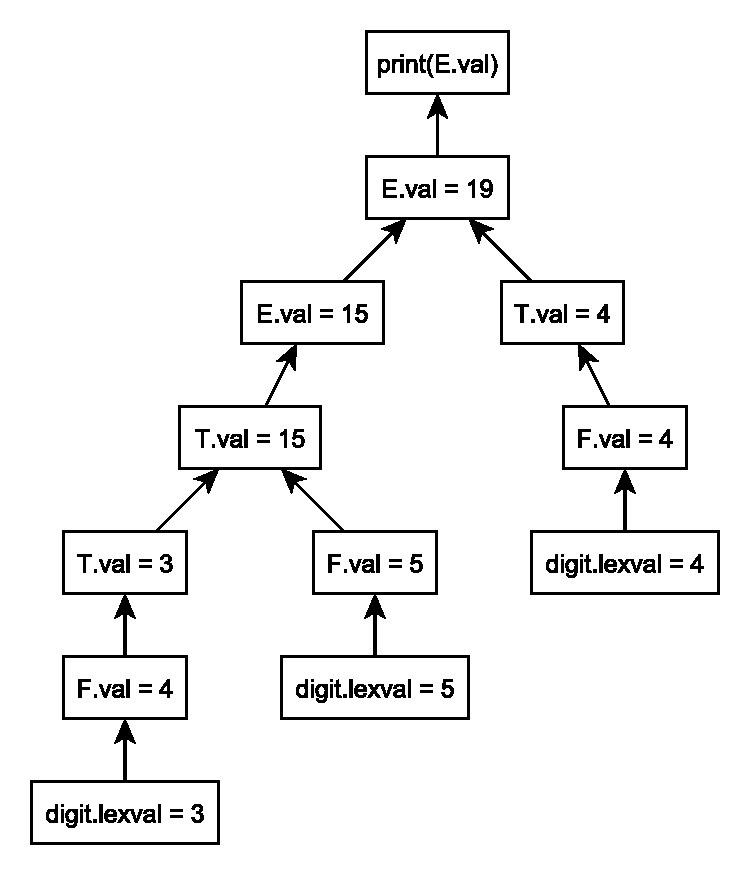
\includegraphics[width=0.6\textwidth]{img/14.pdf}}
    \caption{Dependency trees of S-attributed definitions}
\end{figure}

\subsection{Evaluation Order for S-Attributed Definitions}
S-Attributed definitions can be evaluated in any bottom-up order.
The evaluation order of function post-order (rootNode) corresponds to the order in which a bottom-up parser creates nodes in a parse tree.

\section{Syntax-Directed Translation Schemes (SDT)}
A syntax-directed translation scheme (SDT) is an SDD (syntax-directed definition) with the action of each semantic rule embedded at some position in the right side of the associated production.
\begin{itemize}
    \item an SDT implementation executes each action as soon as all the grammar symbols to the left action are processed;
    \item an SDT having all actions at the right ends of the productions is called ``postfix SDT''.
\end{itemize}

The action $a$ in the rule $A \to X\left\{a\right\}Y$ should be performed:
\begin{itemize}
    \item in bottom-up parsing: as soon as this occurrence of $X$ appears on the top of the parsing stack;
    \item in top-down parsing: just before attempting to expand this occurrence of $Y$ (if $Y$ is non-terminal) or checking for $Y$ on the input (if $Y$ is terminal).
\end{itemize}

\section{Bottom-Up Evaluation of S-Attributed Definitions}
S-attributed SDD can be converted to postfix SDT simply by placing each action at the right end of the associated production.
Action in a postfix SDT can be executed by a bottom-up parser along with reductions.
Example:
\begin{align*}
    L &\to E_n \left\{print(E.val)\right\} \\
    E &\to E_1 + T \left\{E.val = E_1.val + T.val\right\} \\
    E &\to T \left\{E.val = T.val\right\} \\
    T &\to T_1 \ast F \left\{T.val = T_1.val \ast F.val\right\} \\
    T &\to F \left\{T.val = F.val\right\} \\
    F &\to (E) \left\{F.val = E.val\right\} \\
    F &\to digit \left\{F.val = digit.lexval\right\}
\end{align*}

\section{Stack Implementation of Postfix SDT}
Synthesized attributes can be placed along with the grammar symbols on the stack:
\begin{itemize}
    \item when an handle $\beta$ is on top of the stack, all synthesized attributes in $\beta$ have been evaluated;
    \item when the reduction of $\beta$ occurs, the associated actions can be executed.
\end{itemize}
Example:
\begin{align*}
    L &\to E_n \left\{print(stack[top -1].val)\right\} \\
    E &\to E + T \left\{n - top = top - 3 + 1; \right. \\
        &\qquad \left. {} stack[n - top].val = stack[top - 2].val + stack[top].val; \right. \\
        &\qquad \left. {} top = n - top\right\} \\
    F &\to \left\{n - top = top - 3 + 1; \right. \\
        &\qquad \left. {} stack[n - top].val = stack[top - 1].val; \right. \\
        &\qquad \left. {} top = n - top\right\}
\end{align*}

\section{L-Attributed Definitions}
An SDD is L-attributed if any production $A \to X_1 X_2 \ldots X_n$ has:
\begin{itemize}
    \item synthesized attributes;
    \item inherited attributes $X_i.a$ computed in terms of:
    \begin{itemize}
        \item inherited attributes associated with symbol $A$;
        \item inherited or synthesized attributes associated with symbols $X_1 X_2 \ldots i_1$ located at the left of $X_i$.
    \end{itemize}
\end{itemize}

\begin{table}[h]
    \centering
    \begin{tabular}{l|l}
        Productions & Semantic Rules \\ \hline
        $D \to TL$ & $L.inh = T.type$ \\ \hline
        $T \to int$ & $T.type = integer$ \\ \hline
        $T \to real$ & $T.type = real$ \\ \hline
        $L \to L_1, id$ & $L_1.inh = L.inh; addtype(L.inh, id.entry)$ \\ \hline
        $L \to id$ & $addtype(L.inh, id.entry)$
    \end{tabular}
\end{table}

\subsection{Syntax-Directed Translation for L-Attributed Definitions}
To convert an L-attribute SDD to SDT:
\begin{enumerate}
    \item place the actions that compute an inherited attribute for a symbol $X$ immediately before that occurrence of $X$;
    \item place the actions that compute a synthesized attribute at the end of the production.
\end{enumerate}
Example:
\begin{align*}
    D &\to T \left\{L.inh = T.type\right\} \\
    T &\to int \left\{T.type = integer\right\} \\
    T &\to real \left\{T.type = real\right\} \\
    L &\to \left\{L_1-inh = L.inh\right\}L_1, id\left\{addtype(L.inh, id.entry)\right\} \\
    L &\to id \left\{addtype(L.inh, id.entry)\right\}
\end{align*}

\subsection{Bottom-Up Evaluation of L-Attributed Definitions}
A bottom-up parser is aware of the production it is using only when it performs a reduction.
It can therefore execute actions associated with a production only when they are placed at the end of the production.

Actions that compute inherited attributes are not placed at the end of productions.
It is possible to transform an L-attributed definition into an equivalent definition where all actions are placed at the end of productions.

In an L-attributed translation scheme with a rule $A \to X\left\{Y.i = X.s\right\}Y$ where:
\begin{itemize}
    \item $Y.i$ is an inherited attribute defined by a copy rule;
    \item $X.s$ is a synthesized attribute.
\end{itemize}
The value of $X.s$ is already on the parser stack before any reduction to $Y$ is performed.
It can then be retrieved on the stack one position before $Y$ and used anywhere $Y.i$ is called for.
The copy rule $\left\{Y.i = X.s\right\}$ can be eliminated.
Example:
\begin{align*}
    D &\to T \left\{L.inh = T.type\right\}L \\
    T &\to int \left\{T.type = integer\right\} \\
    T &\to real \left\{T.type = real\right\} \\
    L &\to \left\{L_1.inh = L.inh\right\}L_1, id\left\{addtype(L.inh, id.entry)\right\} \\
    L &\to id \left\{addtype(L.inh, id.entry)\right\}
\end{align*}
$$
    \Downarrow
$$
\begin{align*}
    D &\to TL \\
    T &\to int \left\{stack[top].val = integer\right\} \\
    T &\to real \left\{stack[top].val = real\right\} \\
    L &\to L, id \left\{addtype(stack[top - 3].val, stack[top].val)\right\} \\
    L &\to id \left\{addtype(stack[top - 1].val, stack[top].val)\right\} 
\end{align*}

Reaching into the parser stack for an attribute value works only if the grammar allows the position of the attribute value to be predicted.
In the SDT:
\begin{align}
    S &\to aA \left\{C.i = A.s\right\}C \\
    S &\to bAB \left\{C.i = A.s\right\}C \label{eqInterest}\\
    C &\to c \left\{C.s = f(C.i)\right\}
\end{align}
The value of $A.s$ can be either one or two positions in the stack before $C$.
In order to place the value of $A.s$ always one position before $C$, it is possible to insert just before $C$ in rule \ref{eqInterest} a new marker non-terminal $M$ with a synthesized attribute $M.s$ having the same value of $A.s$.
Example:
\begin{align*}
    S &\to aA \left\{C.i = A.s\right\}C \\
    S &\to bAB \left\{C.i = A.s\right\}C \\
    C &\to c \left\{C.s = f(C.i)\right\}
\end{align*}
$$
    \Downarrow
$$
\begin{align*}
    S &\to aA \left\{C.i = A.s\right\} \\
    S &\to bAB \left\{M.i = A.s\right\}M\left\{C.i = M.s\right\}C \\
    C &\to c \left\{C.s = f(C.i)\right\} \\
    M &\to \varepsilon \left\{M.s = M.i\right\}
\end{align*}
$$
    \Downarrow
$$
\begin{align*}
    S &\to aAC \\
    S &\to bABMC \\
    C &\to c \left\{stack[top].val = f(stack[top - 1].val)\right\} \\
    M &\to \varepsilon \left\{stack[top].val = stack[top - 2].val\right\}
\end{align*}

\subsection{Simulating the Evaluation of Inherited Attributes}
In an L-attributed translation scheme with a rule $A \to X\left\{Y.i = f(X.s)\right\}Y$ where:
\begin{itemize}
    \item $X.s$ is a synthesized attribute;
    \item $Y.i$ is an inherited attribute not defined by a copy rule.
\end{itemize}
The value of $Y.i$ is not just a copy of $X.s$ and therefore it is not already on the parser stack before any reduction to $Y$ is performed.
It is possible to insert just before $Y$ a new marker non-terminal $M$ with:
\begin{itemize}
    \item an inherited attribute $M.i = X.s$;
    \item a synthesized attribute $M.s$ to be copied in $Y.i$ and to be evaluated in a new rule $M \to \varepsilon \left\{M.s = f(M.i)\right\}$.
\end{itemize}
Example:
\begin{align*}
    S &\to aA \left\{C.i = f(A.s)\right\}C \\
    C &\to c \left\{C.s = g(C.i)\right\}
\end{align*}
$$
    \Downarrow
$$
\begin{align*}
    S &\to aA \left\{M.i = A.s\right\}M\left\{C.i = M.s\right\}C \\
    C &\to c \left\{C.s = g(C.i)\right\} \\
    M &\to \varepsilon \left\{M.s = f(M.i)\right\}
\end{align*}
$$
    \Downarrow
$$
\begin{align*}
    S &\to aAMC \\
    C &\to c \left\{stack[top].val = g(stack[top - 1].val)\right\} \\
    M &\to \varepsilon \left\{stack[top].val = f(stack[top - 1].val)\right\}
\end{align*}

\subsection{Bottom-Up Evaluation of L-Attributed Definition (bis)}
Systematic introduction of markers makes it possible to evaluate L-attributed translation schemes during bottom-up parsing.
Unfortunately, an $LR(1)$ grammar may not remain $LR(1)$ if markers are introduced.
$LL(1)$ grammars remain $LL(1)$ even when markers are introduced.
Since $LL(1)$ grammars are a proper subset of the $LR(1)$ grammars, every L-attributed translation scheme based on an $LL(1)$ grammar can be parsed in a bottom-up way.